\documentclass[11pt,a4paper]{article}

\usepackage[utf8]{inputenc}
\usepackage[T1]{fontenc}
\usepackage{lmodern}
\usepackage{amsmath,amssymb}
\usepackage{graphicx}
\usepackage{booktabs}
\usepackage[margin=2.5cm]{geometry}
\usepackage{hyperref}

\title{Mean Price in a Lot-Based Inventory Simulation:\\
       A Comparison of Issuing Strategies}
\author{Thomas Kausch}
\date{\today}

\begin{document}
\maketitle

\begin{abstract}
We describe a discrete-event simulation of a single-item inventory with
$(s,S)$ replenishment in which stock is held in lots with individual unit
prices. The rule that decides which lot an item is taken from, the
\emph{issuing strategy}, is a pluggable component. We compare four strategies:
cheapest-first, FIFO, LIFO, and an alternation between the cheapest and the
most expensive lot. The mean price of the items in stock is tracked after every
event. Under cheapest-first issuing it is a biased and therefore unusable
indicator of purchase prices: expensive lots are served last, accumulate in the
stock, and push the mean price towards the upper end of the lot-price
distribution. The other three strategies keep it close to the mean lot price.
\end{abstract}

\section{Model}

The simulation is implemented in Python with SimPy and consists of three
components.

\paragraph{Stock.}
The stock is a set of lots. Each lot $j$ has a quantity $q_j$, a single unit
price $p_j$ shared by all of its items, and an arrival number $a_j$. The
initial stock is one lot whose price equals the expected lot price $\mu_p$.

\paragraph{Demand.}
Demand orders arrive as a Poisson process with rate $\lambda$, i.e.\ with
exponentially distributed inter-arrival times. The size of an order is
$\lceil X\rceil$ with $X\sim\mathcal N(\mu,\sigma^2)$, bounded below by~1.
Each item of an order is taken from a lot chosen by the issuing strategy
(Section~\ref{sec:strategies}). Demand that cannot be served is counted as lost.

\paragraph{Replenishment.}
We use an $(s,S)$ policy with $s=S\,(1-\tau)$, where $\tau$ is the fraction
by which the stock may be empty before a re-order is triggered. After every
demand order, the inventory position (on hand plus on order) is checked. If it
is at or below $s$, an order of size $S-\text{position}$ is placed. It arrives
after an exponentially distributed lead time as \emph{one} lot whose unit
price, the \emph{market price} at the time of purchase, is drawn from
$\mathcal N(\mu_p,\sigma_p^2)$ (truncated at $0.01$).

\begin{table}[ht]
\centering
\begin{tabular}{llr}
\toprule
Symbol & Meaning & Value \\
\midrule
$T$ & simulated time & 800 \\
$\lambda$ & demand arrival rate & 2.0 \\
$\mu,\ \sigma$ & order size mean / std.\ dev. & 5.0 / 2.0 \\
$S$ & order-up-to level (capacity) & 1600 \\
$\tau$ & re-order trigger fraction & 0.25 \\
$s$ & re-order point $S(1-\tau)$ & 1200 \\
 & mean lead time & 5.0 \\
 & initial stock / initial price & 1400 / $\mu_p$ \\
$\mu_p,\ \sigma_p$ & lot price mean / std.\ dev. & 10.0 / 5.0 \\
 & random seed & 42 \\
\bottomrule
\end{tabular}
\caption{Parameters of the simulation runs shown in this paper.}
\label{tab:params}
\end{table}

\section{Computation of the Mean Price}

Let $L(t)$ be the set of lots in stock at time $t$. The number of items and
their total value are
\begin{equation}
  N(t)=\sum_{j\in L(t)} q_j,
  \qquad
  V(t)=\sum_{j\in L(t)} q_j\,p_j ,
\end{equation}
and the mean price per item in stock is
\begin{equation}
  \bar p(t)=\frac{V(t)}{N(t)} .
\end{equation}
The sums are maintained incrementally: when a lot of quantity $q$ and price $p$
arrives, $N\leftarrow N+q$ and $V\leftarrow V+q\,p$; when one item is taken
from lot $j$, $N\leftarrow N-1$ and $V\leftarrow V-p_j$, and an exhausted lot is
removed. After every change the triple $(t,N,\bar p)$ is appended to a history,
so $\bar p$ is a piecewise-constant function of time. When the stock is empty,
$V$ is reset to zero to remove accumulated floating-point error and $\bar p$ is
undefined.

\section{Issuing Strategies}
\label{sec:strategies}

An issuing strategy is a function that, given the lots in stock, returns the
lot from which the \emph{next single item} is taken. Choosing per item rather
than per order makes it possible to split an order across lots according to a
rule. All strategies serve the same demand from the same purchases; only the
choice of lot differs.

\begin{description}
  \item[Cheapest-first.] Take from the lot with the lowest price,
        $\arg\min_j p_j$ (ties: earlier arrival). Expensive lots are touched
        only when all cheaper ones are gone.
  \item[FIFO.] Take from the oldest lot, $\arg\min_j a_j$. The price plays no
        role.
  \item[LIFO.] Take from the newest lot, $\arg\max_j a_j$. The oldest lots
        stay at the bottom of the stack.
  \item[Cheapest/priciest.] Alternate item by item between the cheapest lot
        $\arg\min_j p_j$ and the most expensive lot $\arg\max_j p_j$, so that
        both ends of the price range are drawn down by the same amount. This
        strategy is stateful (it remembers which end is next).
\end{description}

\section{Results}

All runs use the parameters of Table~\ref{tab:params}, the same seed, and
therefore the same 8\,719 demanded items and the same 21 purchases (mean
realised lot price 11.5, maximum 21.7). No demand is lost. Table~\ref{tab:results}
summarises the mean price of the stock, and Figure~\ref{fig:compare} shows its
course for all four strategies together with the market prices of the
purchases.

\begin{table}[ht]
\centering
\begin{tabular}{lrrrr}
\toprule
Strategy & End & Average & Min & Max \\
\midrule
Cheapest-first    & 19.53 & 15.64 & 10.00 & 20.14 \\
FIFO              & 11.22 & 11.37 &  7.27 & 15.11 \\
LIFO              & 10.66 & 10.56 &  8.41 & 13.82 \\
Cheapest/priciest & 10.95 & 11.09 &  9.33 & 13.87 \\
\bottomrule
\end{tabular}
\caption{Mean price $\bar p$ of the stock at the end of the run and its
average, minimum and maximum over all events.}
\label{tab:results}
\end{table}

\begin{figure}[ht]
\centering
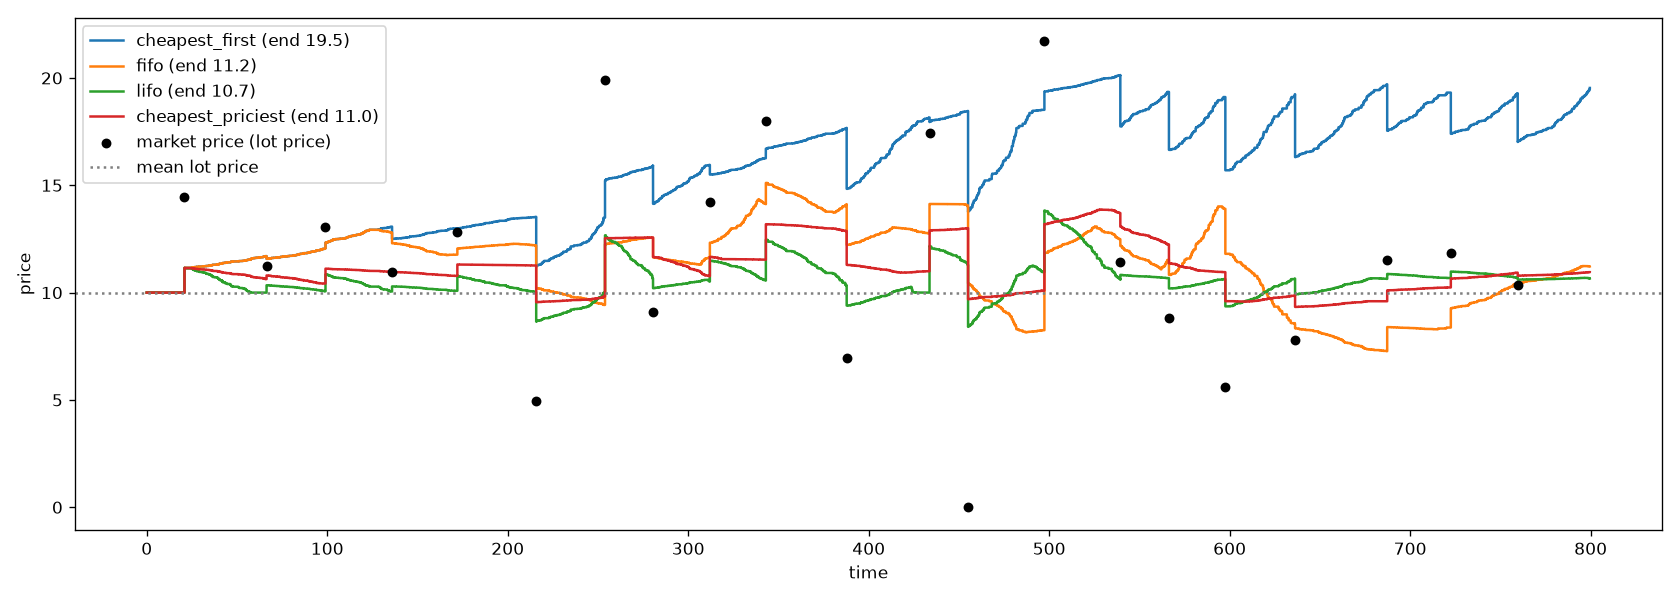
\includegraphics[width=\textwidth]{inventory_sim_compare.png}
\caption{Mean price of the stock under the four issuing strategies. The black
dots are the market prices (lot prices) of the purchases, the dotted line is
the expected lot price $\mu_p=10$.}
\label{fig:compare}
\end{figure}

\paragraph{Cheapest-first.}
Figure~\ref{fig:sim} shows this run in detail. Lot prices are drawn around
$\mu_p=10$, yet $\bar p$ climbs to about $20$, twice the expected purchase
price and close to the maximum lot price. This is a structural consequence of
the rule. A lot is touched only after all cheaper lots are exhausted, and under
an $(s,S)$ policy the stock is refilled long before it is empty (the stock
never fell below 973 of 1600 items). Cheap lots are therefore consumed right
after delivery, while expensive lots stay and form a sediment that dominates
$\bar p$. At the end of the run the stock consists of four lots, priced 11.85,
17.98, 19.88 and 21.71, the last one being the most expensive purchase of the
whole run, delivered at $t\approx 497$ and still untouched.

\begin{figure}[ht]
\centering
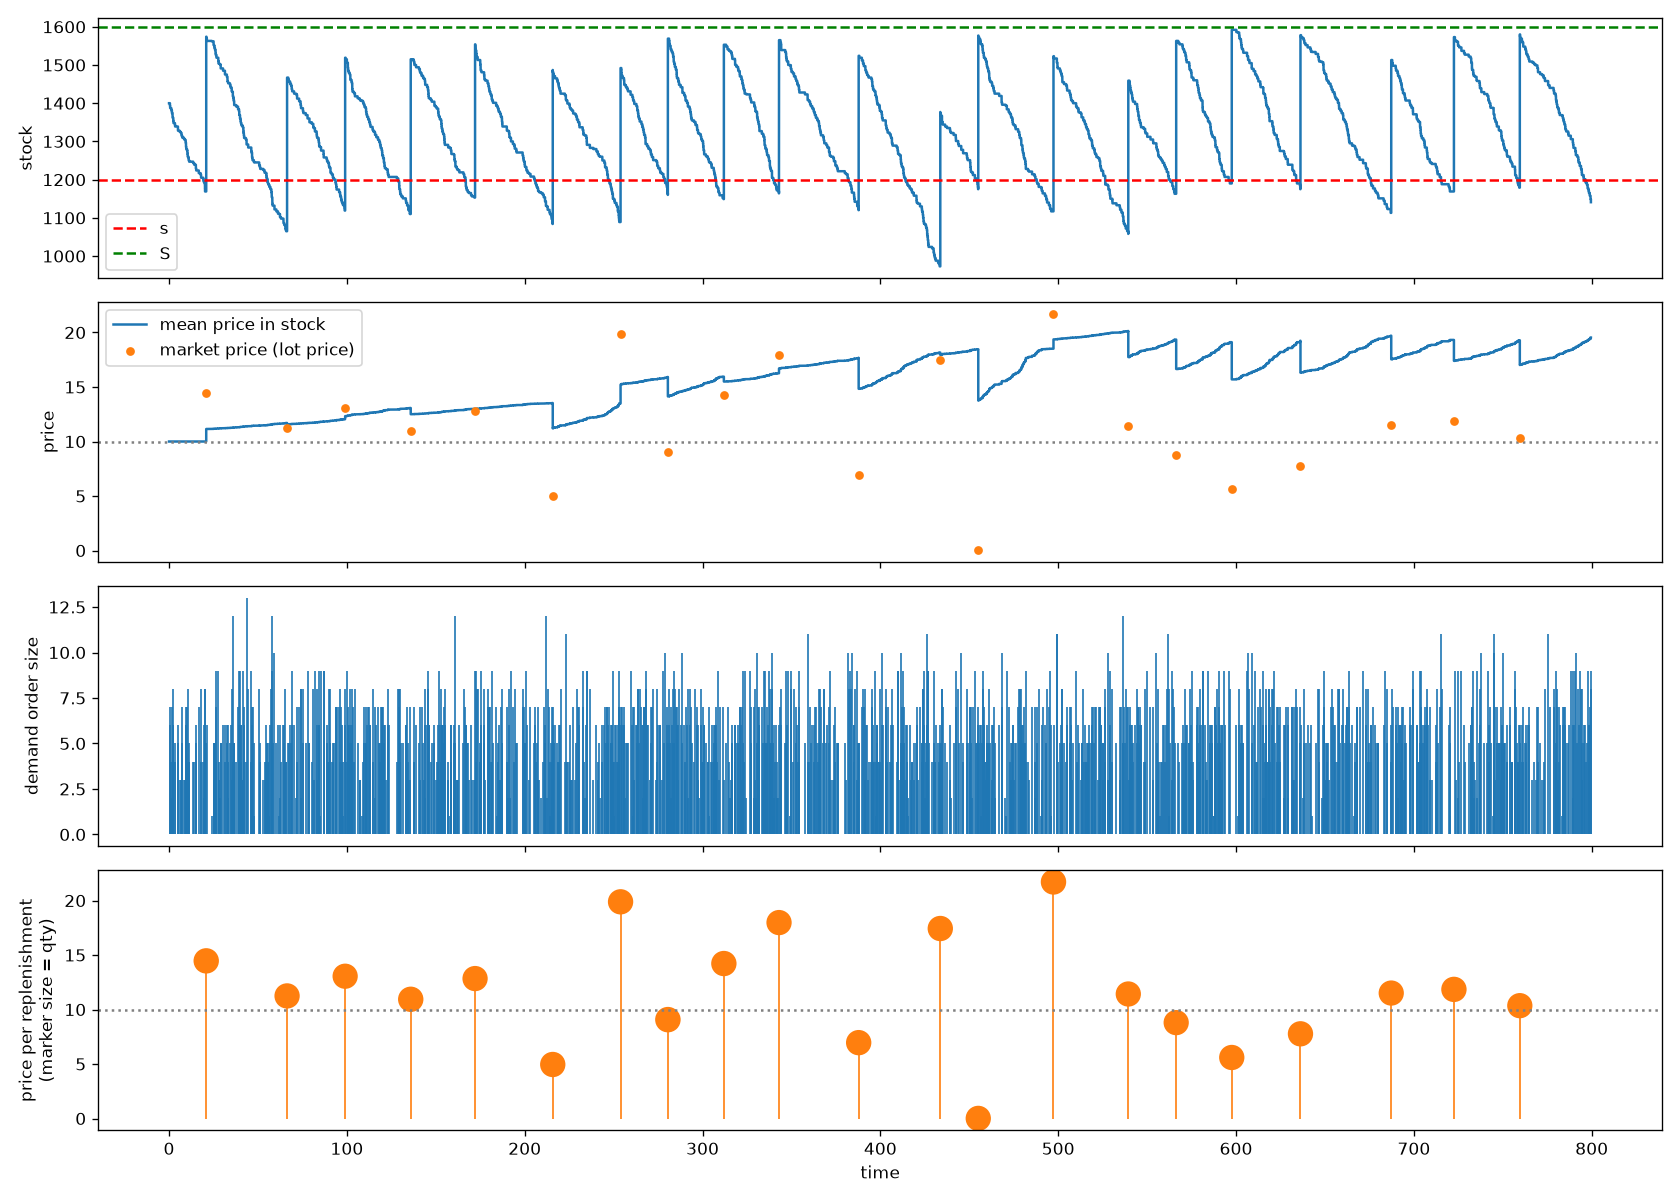
\includegraphics[width=\textwidth]{inventory_sim.png}
\caption{Cheapest-first issuing. From top to bottom: stock level with re-order
point $s$ and capacity $S$; mean price (line) and market prices of the
purchases (dots); demand order sizes; lot prices, marker area proportional to
lot size.}
\label{fig:sim}
\end{figure}

\paragraph{FIFO.}
The oldest lot is always served first, so a lot stays in stock for about one
replenishment cycle, regardless of its price. $\bar p$ follows the recent
purchase prices with a delay and fluctuates between 7.3 and 15.1 around the
expected lot price, without a trend. It ends at 11.22, close to the realised
mean lot price of 11.5.

\paragraph{LIFO.}
The newest lot is served first, so the stock is split into a small, quickly
turning top and an untouched bottom. Because the initial lot was priced at
$\mu_p$, the untouched bottom (973 items at 10.00 at the end) happens to sit
exactly at the expected price, and $\bar p$ has the smallest spread of all
strategies (8.4 to 13.8, end 10.66). This is an artefact of the initial price:
with an initial lot at 15 instead of 10, the same run ends at 14.9. LIFO thus
freezes whatever lots happen to be at the bottom, here the initial lot.

\paragraph{Cheapest/priciest.}
Drawing equal amounts from both ends removes the sediment at the expensive end
as well as the cheap lots. $\bar p$ stays between 9.3 and 13.9 and ends at
10.95, the narrowest range together with LIFO, and, unlike LIFO, without
depending on the initial lot, because both extremes are consumed.

\section{Consequences}

Under cheapest-first issuing the mean price of the stock is a
\emph{survivorship-biased} quantity: it describes the items that nobody wanted
to take, not the items that were bought.
\begin{itemize}
  \item It is \textbf{not an estimator of the purchase price}: its long-run
        value depends on the number of purchases and the spread $\sigma_p$,
        not on $\mu_p$.
  \item It is \textbf{not usable as a valuation or cost basis} for the issued
        items, since these are by construction the cheapest ones.
  \item It is \textbf{not a stable state variable}: it trends with simulation
        length and depends on single expensive lots.
  \item It carries \textbf{no information about the current market price} and
        cannot drive re-ordering or pricing decisions.
\end{itemize}
FIFO, LIFO and cheapest/priciest do not have this drift, because they do not
let one price class accumulate in the stock. They are not equally robust,
though. FIFO and cheapest/priciest depend only on the recent purchases, while
LIFO depends on the lots left at the bottom of the stack, here the initial lot.

\paragraph{Limits.}
A balanced mean price does not guarantee a profit. Items taken from expensive
lots, as under cheapest/priciest, are sold with a low margin or at a loss if
the selling price does not follow the purchase price. Fixing the bias of the
statistic therefore opens a second question, the profitability of the rule.

\paragraph{Lesson learned.}
In reality the mean price influences the selling price and with it the demand.
Here demand is independent of the price: $\lambda$ and the order size are
constants. A realistic model must close this loop and describe demand as a
function of the (mean) price, for example $\lambda=\lambda(\bar p)$. Only then
can the issuing strategies be compared by their effect on sales volume and
profit and not only by the mean price they produce.

\section{Conclusion}

We presented a lot-based inventory simulation with $(s,S)$ replenishment and a
pluggable issuing strategy, and the incrementally maintained mean price
$\bar p=V/N$. Cheapest-first issuing gives this measure a systematic upward
bias: expensive lots are never consumed, remain in stock, and drive $\bar p$
towards the maximum lot price (19.5 against an expected 10). FIFO, LIFO and the
alternation between the cheapest and the most expensive lot keep it between
about 7 and 15 around the expected lot price. The problem is therefore not the
mean price itself but the decision to always serve from the cheapest lot, and
the resulting property cannot be used as a price indicator. A comparison of
the strategies by profit requires price-dependent demand and a selling price,
which the present model does not have.

\end{document}
